\chapter{Introduction}

	\section{Contexte}

		\paragraph{Développement logiciel \\}
		
			Le contexte de cette thèse se focalise sur le monde et l'environnement de développement logiciel au coeur de l'informatique. L'\Gls{open source} aujourd'hui, peut s'étendre aux oeuvre de l'esprit dont il ne sera pas traité particulièrement mais désignera les logiciels dit "ouverts".
		
		\subsection{Introduction à l'open source}

			Afin de lever l'ambiguïté entre les logiciels "libres" (en anglais "free", pouvant désigner un logiciel gratuit, ou libre) et les logiciels "ouverts", l'expression "\gls{open source}" est apparue en 1998 par Christine \bsc{Peterson} du Foresight Institute.
			Richard \bsc{Matthew Stallman} défend le terme de \textit{free software} à travers son organisme la \acrfull{fsf}
			Eric \bsc{Raymond} et Bruce \bsc{Perens} créent en 1998, l'\acrfull{osi}, qui délivre le label "\acrshort{osi} approved" aux licences qui satisfont aux critères définis dans l'Open Source Definition.

			\begin{center}
				\textit{
				\textquote{
					L'Open Source permet une méthode de développement de logiciels qui exploite la puissance de l'évaluation par les pairs distribuée et la transparence des processus. La promesse de l'open source est une meilleure qualité, une meilleure fiabilité, une plus grande flexibilité, des coûts moins élevés et la fin de l'immobilisme prédateur des fournisseurs.} - \acrshort{osi}
				}
			\end{center}

			Un logiciel \textit{libre}, ou logiciel \textit{open source}, est un programme dont le code source est distribué et peut être utilisé, copié, étudié, modifié et redistribué sans restriction.

			Les deux appellations «open source» et «logiciel libre» sont presque équivalentes, mais correspondent à des écoles de pensées différentes. Libre ne signifie pas gratuit.
			Rien n'interdit de faire payer le logiciel bien que l'utilisateur en fonction de la licence pourra le redistribuer librement, on considère donc qu'un logiciel open source est généralement gratuit.
				
		\paragraph{Pourquoi je vous parle de l'open source ?\\}

			L'open source est un outil capital dans le monde de l'informatique.
			En tant que développeur j'ai découvert l'open source au sein de mon entreprise actuelle, Docdoku.
			Docdoku développe un logiciel open source aidant de nombreuses entreprises.

			Bien qu'important il n'est pourtant que vaguement évoqué et méconnu.
			Voici deux affirmations erronées qui planent sur l'open source 
			
			\subparagraph{« L'open source c'est moins bien »\\}

				L'open source est souvent associé à de mauvais termes. On peut entendre logiciel gratuit, libre, non supporté par une entreprise, développé par le particulier ou des communautés en tant que passe-temps. Un manque de rigueur peux donc s'en dégager et dévaloriser l'image de celui-ci auprès des éditeurs et consommateurs.

			\subparagraph{« L'open source n'a pas besoin de moi »\\}

				L'open source ne se résume pas seulement au développement de code informatique et est un vaste domaine ou chaque individu, quelque soit ses compétences, peut y participer afin de rendre le monde et l'informatique meilleure qu'elle n'est.\\

			Malgré le projet que développe notre entreprise sous open source, je n'ai pas réussis à obtenir des réponses concrètes sur ce qu'est l'open source, ce que cela implique, auprès de mes collègues de travail et de formation. A ceci, l'on peut ajouter que pour beaucoup, l'open source est signe de stabilité, fiabilité, sécurité.\\

			En plus du manque de connaissance sur le sujet de moi-même et mon entourage, je constate ainsi qu'il existe encore beaucoup d'amalgames autour de l'open source, des défauts et abus de langage.\\
			Les institutions et entreprises que j'ai pu fréquenté dans le monde de l'informatique ne sensibilisent pas assez les développeurs actuels et en devenir sur l'open source. Les avantages qu'offrent celui-ci, l'aspect juridique, les conditions d'utilisation et bien d'autres caractéristiques propres à l'open source ne sont pas enseignés.\\

			Je pars donc du principe que l'open source ne fait pas assez de "bruit" dans le monde, ainsi je souhaite développer à travers cette thèse, l'intrigation, la passion et l'envie de nous tourner vers l'open source, d'y contribuer et d'en faire la solution privilégiée des développeurs et des consommateurs occasionnels en me positionnant du coté des éditeurs.

		\subsection{De l'importance de l'open source}

				Une étude auprès de 950 entreprises dans l'informatique a été réalisé en 2019 par la fondation Redhat qui a permis de statuer sur l'évolution de l'open source. La moitié de ces entreprises sont situés aux États-Unis, le reste est répartie entre l'Asie Pacifique, le Royaume-Uni et l'Amérique Latine.

				\paragraph{L'open source à travers le monde\\}

					L'open source est utilisé par beaucoup de personnes et ce à travers le monde selon une étude (voir Annexe 1) sur la diffusion du libre à travers les frontières.
					Son utilisation est versatile, la moitié des entreprises interrogé l'utilise pour différents secteurs 

					\begin{itemize}[label=\textbullet, font=\LARGE \color{burntorange}]
					\item Modernisation des infrastructures
					\item Transformation digitale
					\item Développement d'applications
					\item DevOps
					\item Intégration dans les applications
					\item Modernisation des applications
					\end{itemize}

				\paragraph{Les domaines informatique de l'open source dans l'entreprise\\}

					Les nouveau domaines du numérique en vogue ainsi que certains reservés auparavants aux logiciels propriétaire s'ouvrent sur l'open source. Ceci inclus notemment les outils de gestion du cloud, security, la sécurité, les données analysées, et le stockage (Voir annexe 2)

				\clearpage
				\paragraph{Les réticences encores présente sur l'open source\\}

					Malgré l'impact bénéfique de l'open source pour les entreprises, il reste encore quelques inquiétudes planant au dessus de l'open source et des réticence à son utilisation généralisée.

					\begin{figure}[h]
						\center
						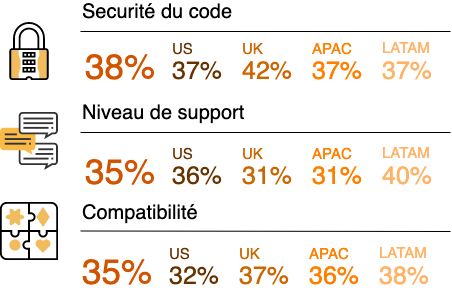
\includegraphics[scale=0.70]{./img/Barreer_os.png}
						\caption{Causes principales des réticences à l'open source}
						\caption*{\color{silver}Source: redhat.com}					
					\end{figure}										

					J'en conclus donc qu'à travers le hack et le piratage de produit open source, les entreprise positionnent la sécurité de l'open source comme une inquiétude majeure.

				\paragraph{L'évolution de l'utilisation de l'open source\\}

					Beaucoup d'entreprises continuent tout de même à utiliser des logiciels propriétaires, mais cette tendance tend à diminuer sur les 2 prochaines années. Ceci grâce aux nouvelles technologies provenant du \gls{web 3.0}, notemment la \gls{conteneurisation}, qui est considéré comme un brassage de produit collaboratif open sources. De nombreuses entreprise aujourd'hui se tourne vers des solutions de conteneurisation, due à l'open source.
					
					\begin{figure}[h]
						\center
						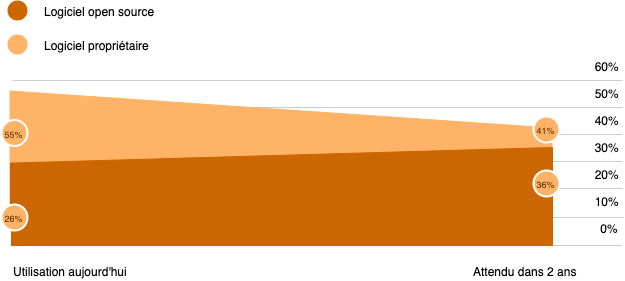
\includegraphics[scale=0.60]{./img/osinentreprise.png}
						\caption{Évolution de l'open source dans les années à suivre}
						\caption*{\color{silver}Source: redhat.com}					
					\end{figure}
					\clearpage

	\section{Problématique}
		\paragraph*{}

			Je vais donc vous présenter la problématique suivante :
			\begin{center}
				\begin{displayquote}
					\textbf{Comment valoriser, en tant qu'éditeur, l'open source et en faire la solution privilégiée des consommateurs ?}
				\end{displayquote}
			\end{center}

		\paragraph*{}
			
			Afin de répondre à cette problématique, je vais m'appuyer sur des hypothèses fondées sur mon vécu en entreprise mais également issues de ma réflexion personnelle dans mon métier de développeur logiciel.

	\section{Hypothèses}

		\paragraph{Les plateformes promotrices\\}

			Selon moi si le nombre de plateforme hébergeant du contenu open source et offrant la possibilité d'y contribuer mettaient plus en avant les projets open source, par une démarche plus marketing et publicitaire,utilisation d'images, présentation du projet par une vidéo, l'open source serait plus prisé par les consommateurs et l'on constaterait plus de contributions à ces projets.

		\paragraph{L'optimisation\\}

			Si nous améliorons l'aspect communautaire dans son organisation, donnons accès à des formations, inclure et impliquer un peu mieux les personnes sans pour autant compliquer la participation à celle-ci, nous valoriserons l'open source.

		\paragraph{Les envies et besoin des consommateurs\\}

			Si les consommateurs possédait des moyens efficaces afin d'exprimer leur souhaits et besoins en terme d'open source, ils en seraient plus satisfait et cela en ferait la solution idéale à leurs yeux.

	\section{Méthodologie de travail / périmètre}
		\paragraph{Etude de l'open source}

			\subparagraph{Présentation de l'open source\\}

				Afin d'avoir un retour sur mes hypothèses, il m'est nécessaire d'avoir une meilleure vision d'ensemble de l'open source et un périmètre défini.

			\subparagraph{Les éditeurs open source\\}

				Je me positionne du côté des éditeurs, pour diverses raisons évoqués précédemment, je souhaite donc en savoir plus sur l'éditeur, ses rôles, son périmètre d'action.

			\subparagraph{L'optimisation des ressources\\}
		
				Après avoir fait la lecture et l'analyse personnelle de plusieurs ouvrages dont 2 principaux sur lesquels je m'appuyerai : 
		
				\begin{displayquote}
					\textquote{Réfléchissez et devenez riche} - Napoleon \bsc{Hill} - 1937
				\end{displayquote}
				\begin{displayquote}
					\textquote{Oser la confiance} - Bertrand \bsc{Martin} (†), Vincent \bsc{Lenhardt}, Bruno \bsc{Jarrosson} - 1996
				\end{displayquote}
		
				Je souhaite effectuer des recherches sur l'optimisation (et ses moyens) des ressources qui définissent l'open source.

			\subparagraph{Le consommateur\\}
				En étudiant le consommateur, nous verrons les besoins et activités relatives à l'open source.

			\subparagraph{Le marché de l'open source\\}
				Enfin nous verrons l'aspect économique associé à l'open source en étudiant son marché.

		\paragraph{Sur le terrain \\}
			Lors de mon étude terrain je consoliderai mes recherches dans les domaines cités précédemment pour pouvoir les confronter.

		\paragraph{L'analyse et les résultats \\}
			Je transposerai alors mes études et relevés afin de valider ou réfuter mes hypothèses et apporter une réponse acceptable à ma problématique en guise de conclusion.